\documentclass[%
  a4paper,oneside,%
  %arial,
  11pt,% <10pt, 9pt>
  smallchapters,
  %style=screen,
  %sender=bottom,
  green,% <orange, green, violet>
  rgb, <cmyk>
  %mono
  ,]{tubsbook}
  
\usepackage{siunitx}
\sisetup{load-configurations = abbreviations}  
  
\usepackage{listings}  % for code stuff
\usepackage{minted}

\usepackage{physics}

\usepackage{bbm} %for probability notation

\usepackage{xcolor}

\definecolor{codegreen}{rgb}{0,0.6,0}
\definecolor{codegray}{rgb}{0.5,0.5,0.5}
\definecolor{codepurple}{rgb}{0.58,0,0.82}
\definecolor{backcolour}{rgb}{0.95,0.95,0.92}

\lstdefinestyle{mystyle}{
	language=Python,
    backgroundcolor=\color{backcolour},   
    commentstyle=\color{codegreen},
    morekeywords={self},
    keywordstyle=\color{magenta},
    numberstyle=\tiny\color{codegray},
    stringstyle=\color{codepurple},
    basicstyle=\ttfamily\footnotesize,
    breakatwhitespace=false,         
    breaklines=true,                 
    captionpos=b,                    
    keepspaces=true,                 
    numbers=left,                    
    numbersep=5pt,                  
    showspaces=false,                
    showstringspaces=false,
    showtabs=false,                  
    tabsize=2
}


\newcommand\pythonstyle{\lstset{
	language=Python,
    backgroundcolor=\color{backcolour},   
    commentstyle=\color{codegreen},
    morekeywords={self},
    keywordstyle=\color{magenta},
    numberstyle=\tiny\color{codegray},
    stringstyle=\color{codepurple},
    basicstyle=\ttfamily\footnotesize,
    breakatwhitespace=false,         
    breaklines=true,                 
    captionpos=b,                    
    keepspaces=true,                 
    numbers=left,                    
    numbersep=5pt,                  
    showspaces=false,                
    showstringspaces=false,
    showtabs=false,                  
    tabsize=2
}}


% Python environment
\lstnewenvironment{python}[1][]
{
\pythonstyle
\lstset{#1}
}
{}




%lstset{style=mystyle}

\usepackage{bm} 
\usepackage{amsmath}
 
\renewcommand{\familydefault}{\sfdefault}
\usepackage[utf8]{inputenc}
\RequirePackage{scrlfile}
\ReplacePackage{scrpage2}{scrlayer-scrpage}

\usepackage[ngerman,english]{babel}

\usepackage{lipsum} % Blindtext-Paket
\definecolor{InAGreen}{RGB}{172,193,58}

% Titelseiten-Elemente
\title{A Statistical Approach for the Fusion of Data and
Finite Element Analysis in Vibroacoustics}
\subtitle{Untertitel}
\author{Lucas Hermann}
%\logo{Institut fuer Lorem Ipsum}
\logo{
\includegraphics{InA-Logo-rgb.pdf}}
\titleabstract{\lipsum[2]}
\titlepicture{infozentrum.jpg}
% Rückseiten-Elemente
\address{%
  Herr Mustermann\\
  Schlossallee 1\\
  33333 Darmstadt}
\backpageinfo{%
  \lipsum[5]
}
\usepackage{pdfpages}								% Einbinden von PDF-Pages
\usepackage[colorlinks,pdfpagelabels,pdfstartview = FitH,bookmarksopen = true,bookmarksnumbered = true,linkcolor = black,plainpages = false,hypertexnames = false,citecolor = black] {hyperref}
\usepackage[figure]{hypcap} 
\bibliographystyle{ieeetr}

\begin{document}

%\maketitle[image,logo=left]%[<plain/image/imagetext>,<logo=left/right>]
%\makebackpage[trisec]%[<plain/info/addressinfo>]
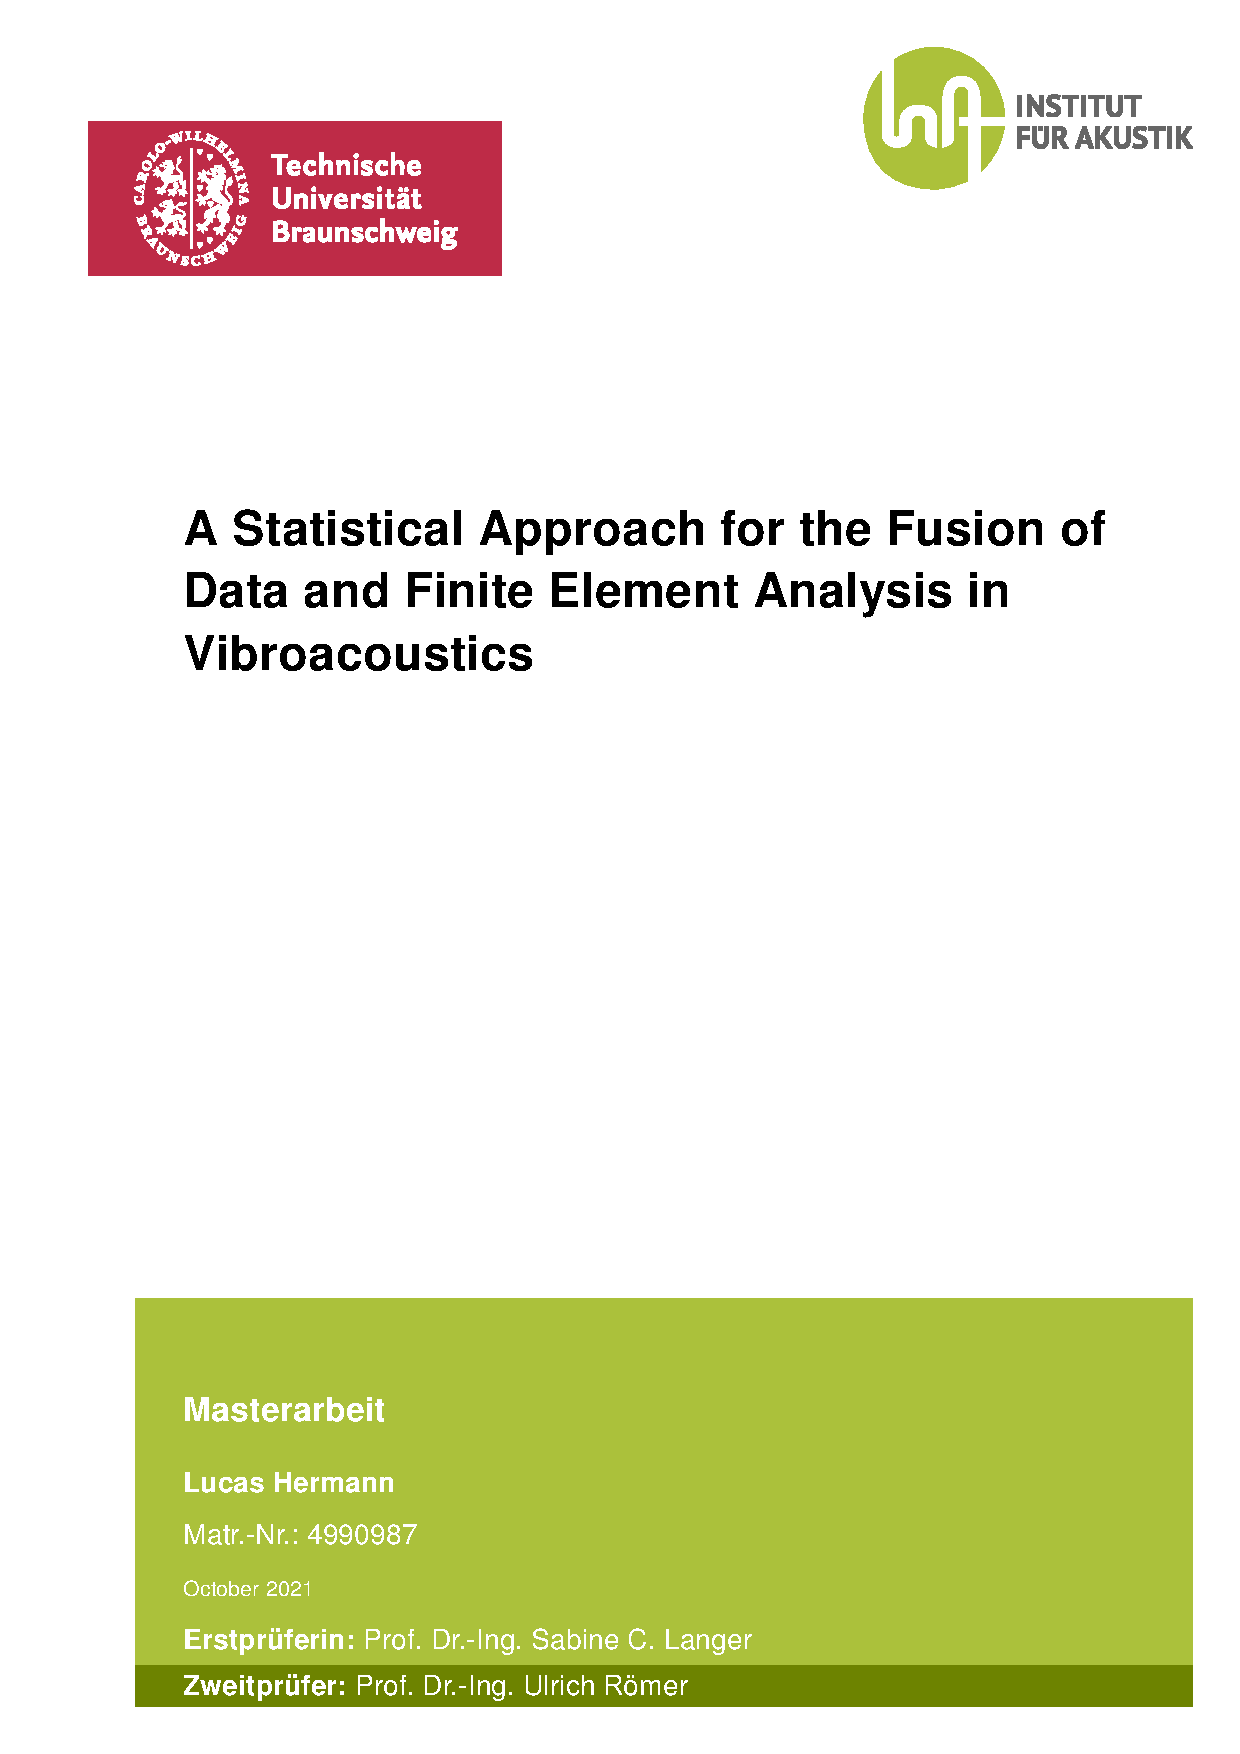
\includepdf[pages=-]{./Deckblatt/2099_StA_Name_Deckblatt.pdf}

\chapter*{Declaration}
Hiermit versichere ich, Lucas Hermann, durch meine Unterschrift, dass ich die
vorliegende Masterarbeit mit dem Titel ``<<Titel>>'' selbständig und ohne Benutzung
anderer als der angegebenen Hilfsmittel angefertigt habe. Alle Stellen, die wörtlich oder sinn-
gemäß aus veröffentlichten oder unveröffentlichten Schriften entnommen sind, habe ich als
solche kenntlich gemacht. Insbesondere sind auch solche Inhalte gekennzeichnet, die von
betreuenden wissenschaftlichen Mitarbeiterinnen und Mitarbeitern des Instituts für Akustik eingebracht wurden.

Die Arbeit oder Auszüge daraus haben noch nicht in gleicher oder ähnlicher Form dieser
oder einer anderen Prüfungsbehörde vorgelegen.

Mir ist bewusst, dass Verstöße gegen die Grundsätze der Selbstständigkeit als Täuschung
betrachtet und entsprechend der Prüfungsordnung geahndet werden.

\begin{flushright}
Braunschweig, \today
\end{flushright}

\vspace{2cm}
\hspace{2cm}\rule{5cm}{1pt}

\hspace{2cm}\small{Lucas Hermann} 

\chapter*{Abstract}
\lipsum[1]

\tableofcontents


\chapter{Introduction}

\textcolor{tubsSecondary}{Dies ist ein Text in \texttt{tubsSecondary}.}
\textcolor{tubsViolet}{Dies ist ein Text in \texttt{tubsViolet}.}
\textcolor{tubsGreenDark}{Dies ist ein Text in \texttt{tubsGreenDark}.}\bigskip

\lipsum[1]

\begin{itemize}
  \item Aufzählungspunkt Eins
  \item Aufzählungspunkt Zwei
    \begin{itemize}
      \item Unter-Aufzählungspunkt Eins
      \item Unter-Aufzählungspunkt Zwei
    \end{itemize}
  \item Aufzählungspunkt Drei
\end{itemize}



\chapter{FEM Solution of the Helmholtz Equation}
An acoustic field is represented by the wave equation. It returns the acoustical pressure at a point in space $X$ for a certain frequency and time.
The Helmholtz equation describes the wave equation in a time-independent manner. It has a dependency on the frequency, so the goal is to solve the Helmholtz equation for a range of frequencies in order to obtain a frequency response plot which gives insight on the modal behaviour of the system.

\section{Wave Equation and Helmholtz Equation}
In Vibroacoustics there are usually two coupled domains: At first, there is some kind of solid medium which emits sound. The movement of that solid can be described within the field of elastodynamics using the Bernoulli or Timoshenko beam theory in 1D or, for the 2D case of plates, Kirchhoff or Reissner Mindlin plate theory. The focus of this thesis is another: As soon as the sound is emitted from the solid, the Wave equation is used to describe the motions of sound waves through a liquid or gas, such as air. 
The following closely follows [Mats G Larson FEM] and [Möser].
The behaviour of a gas in a domain $\Omega$ can be described using the density $\rho$, the pressure $p$ and the velocity $v$. By changing the velocity or pressure locally by e.g. a speaker or a vibrating plate, this change is propageted through the medium: One can think of the gas as a system of infinitesimally small spring-mass systems. Deflecting one spring yields in a deflection of the adjacent spring, or gas volume, but time-delayed due to the gas's inertia. That leads to a wave propagating through the medium. 
Newton's second law states that mass times accelaration equals force. If a gas volume is accelerated in one direction, that leads to a force on the neighbouring particle [Möser]
%
\begin{equation}
m \dot{v} = S  \left[  p(x) -p(x + \Delta x)  \right] 
\end{equation}
with $m$ the mass of the gas volume, $S$ the surface the two volume's contact area and $\Delta x$ the length of a gas volume in the direction of motion. Considering $m = \Delta x S \rho$ there holds
\begin{equation}
\rho \dot{v} = - \frac{p(x) -p(x + \Delta x)}{\Delta x} \; .
\label{eqn:waveEqDeriv1}
\end{equation}
Assuming interaction between infinitessimaly small gas particles and therefore taking the limit of the difference quotient in \ref{eqn:waveEqDeriv1} yields the differential quotient and hence
\begin{equation}
\rho \dot{v} = - \nabla p \;.
\label{eqn:Tragheitsges}
\end{equation}

If a volume is expanded, the pressure of the contained gas drops and vice versa. Therefore a change of volume is proportinal to a negative change of pressure. An expanding volume is also represented by the divergence of the velocity.[Larson FEM] Imagine quickly pulling a piston out of an airtight cylinder: The air particles will move in the direction of the piston movement while the volume expands and the pressure drops. Hence, there holds
\begin{equation}
\dot{p} = -k \nabla v
\label{eqn:Constit}
\end{equation}
with $k$ a proportionality constant dependent on the medium.
Differentiating \ref{eqn:Constit} after $t$ yields 
\begin{equation}
\ddot{p} = -k \nabla \dot{u} \;.
\end{equation}
Inserting \ref{eqn:Tragheitsges} and considering $c^2 = k/\rho$ there holds for the acoustic Wave equation
\begin{equation}
\ddot{p} = c^2 \nabla^2 p 
\label{eqn:WaveEq}
\end{equation}
which involves derivations in both time and space. To obtain a general representation of the behaviour of a pressure field independent of time, the Helmholtz equation can be derived as follows.
Considering a separation ansatz [Westermann]
\begin{equation}
p(x,t) = X(x) \cdot T(t) \; ,
\end{equation}
there holds for \ref{eqn:WaveEq}

\begin{align}
X(x) \cdot \pdv[2]{T(t)}{t} &= c^2 \nabla^2 X(x) \cdot T(t)\\
\frac{1}{T(t)} \pdv[2]{T(t)}{t} &= c^2 \frac{1}{X(x)} \nabla^2 X(x) = const. = - \omega^2 \; .
\end{align}
With the wave number $k = \omega / c$ 
\begin{equation}
\nabla^2 X(x) + k^2 X(x) = 0
\end{equation}
is the Helmholtz equation which is a representation of the wave equation independent of time [Mathebuch Helmholtz].
%
In the following it is going to be referred to by
\begin{equation}
\nabla^2 p + k^2 p = 0
\label{eqn:Helmholtz}
\end{equation}
with $p [\SI{}{\pascal}]$ the pressure field and $k$ the wave number. $k$ is defined as \begin{equation}
k = \frac{\omega}{c_0} = \frac{2 \pi f}{c_0}
\end{equation}
with $\omega$[\SI{}{\radian}] the angular frequency, $f$[\SI{}{\per\s}] the frequency and $c_0[\SI{}{\metre\per\s}]$ the speed of sound in the considered medium.
(\ref{eqn:Helmholtz}) is solved as a boundary value problem.
\section{Boundary Conditions}
[ATALLA]
\paragraph{Dirichlet}
The Dirichlet boundary condition for the Helmholtz equation is simply a prescribed pressure at the $\Gamma_D$ part of the boundary:
\begin{equation}
p = \bar{p}
\end{equation}


\paragraph{Neumann}
The Neumann boundary condition at $\Gamma_N$ reads
\begin{equation}
\dv{p}{n} = \rho \omega^2 \bm{U} \cdot \vec{n}
\end{equation}
with $\bm{U}$ the displacement and $\vec{n}$ the normal direction of the surface. It can be thought of as a piston moving with circular frequency $\omega$ at the boundary which created a velocity and pressure change. Choosing a Neumann BC $\Gamma_N = 0$ resembles a reflecting boundary.

\paragraph{Robin}
The Robin or impedance boundary condition at $\Gamma_R$ reads
\begin{equation}
\dv{p}{n} + ik \beta p = 0
\end{equation}
with $\beta$ the specific normalized acoustic admittance.
Figure \ref{fig:BCEx} shows an example on where boundary conditions could be applied on a 2D domain. Figure \ref{fig:BCTh} shows the approach chosen in this thesis.


\begin{figure}[h]
\begin{center}
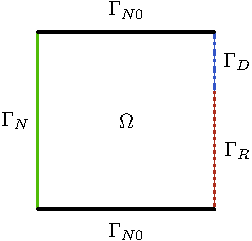
\includegraphics[width=0.4\textwidth]{pics/BCsExample}
\caption{Boundary Conditions of diffrent type can be arranged on the boundary. In this example, the left side is a Neumann boundary, the upper and lower boundaries are totally reflecting and the right side consists of an impedance BC and a Dirichlet BC.}
\label{fig:BCEx}
\end{center}
\end{figure}


\begin{figure}[h]
\begin{center}
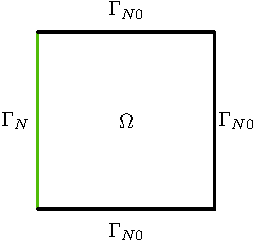
\includegraphics[width=0.4\textwidth]{pics/BCsThesis1}
\caption{Boundary Conditions of the problem for this thesis. A Neumann boundary is applied on the side of the domain. The rest of the boundary is considered as reflecting, i.e. $\Gamma_N = 0$.}
\label{fig:BCTh}
\end{center}
\end{figure}

Using FEniCS, the boundary conditions can be applied to the system of equations by 
%
\begin{minted}
[
frame=lines,
framesep=2mm,
baselinestretch=1.2,
bgcolor=backcolour,
fontsize=\footnotesize,
linenos
]
{python}
class BoundaryX_L(SubDomain):
	self.tol = 1E-14
	def inside(self, x, on_boundary):
		return on_boundary and near(x[0], 0, tol)# and (x[1] < 0.3)

class BoundaryX_R(SubDomain):
	def inside(self, x, on_boundary):
		return on_boundary and near(x[0], 1, tol)# and (x[1] < 0.3)

boundary_markers.set_all(9999) # all markers default to zero.
bxL = BoundaryX_L()
bxR = BoundaryX_R()
bxL.mark(boundary_markers,0) # left side is marked as "0"
bxR.mark(boundary_markers,1) # right side is marked as "1"

ds = Measure('ds', domain=self.mesh, subdomain_data=boundary_markers) #define a new operator for the boundary
\end{minted}
%
%
This construction can then be used when defining the variational problem:
%
\begin{minted}
[
frame=lines,
framesep=2mm,
baselinestretch=1.2,
bgcolor=backcolour,
fontsize=\footnotesize,
linenos
]
{python}
U = 0.0001 #Piston displacement
g = self.rho * self.omega**2 * U
a = inner(nabla_grad(self.u), nabla_grad(self.v))*dx - self.k**2 * inner(self.u,self.v)*dx #variational Problem
L = (self.v*g)*ds(0) # 0 is the chosen boundary marker
\end{minted}


Dirichlet boundary conditions can be applied after assembling the system by 
\begin{minted}
[
frame=lines,
framesep=2mm,
baselinestretch=1.2,
bgcolor=backcolour,
fontsize=\footnotesize,
linenos
]
{python}
def boundaryDiri(x):
	return x[0] > (1.0 - DOLFIN_EPS) and x[1] < 0.0 + DOLFIN_EPS
self.bcDir = DirichletBC(self.V, Constant(0.0), boundaryDiri)
A = assemble(a)
b = assemble(L)
self.bcDir.apply(A, b)
\end{minted}

\section{Weak Formulation and Discretisation}
Explain what the weak form is and why we need it. 
Derive the weak form, completely with integration by parts etc. explain all parts of it and what they represent.

explain what a bilinear and a linear form is!


Eq. (\ref{eqn:Helmholtz}) is considered a \emph{strong}	formulation. In order to be able to set up the FEM, the PDE needs to be in the \emph{weak} form. Among other possibilities, the weak form can be derived using the Weighted Residuals Method.

In order to lower the degree of derivation, integration by parts is executed:







\section{The Classical Finite Element Method}


The Finite Element Method (FEM) is a procedure which makes it simple to approximately solve partial differential equations (PDEs) which would be very hard or even impossible to solve analytically. As the name suggests, the calculation domain is split into $n_e$ individual elements on which the PDE is approximated using so-called Ansatz functions. The process of dividing the domain in $n_e$ elements is called discretization. The polynomial degree of the Ansatz functions and the number of elements determine the accuracy of the approximation. In order to set up the FEM, the PDE needs to be in the so-called variational, or "weak", formulation. 
After discretization of the domain and deriving the weak formulation, it can be approximated on the individual elements. Assembling the element matrices yields a global system of equations which can, after boundary conditions are applied, be solved for the unknown vector.


\subsection{Integral and Weak Formulation}
The Helmholtz Equation is the so-called governing equation for the problem considered in this thesis. The governing equation is given in the strong form and is usually of higher order. This property makes it hard to solve the equation, both analytically and numerically. For being able to apply the FEM, the order of the PDE has to be lowered. That is archieved by first bringing the equation in the weak, or also variational, formulation.
Bringing the governing equation in the weak form can be accomplished using the Method of Weighted Residuals. 
\paragraph{The Weigthed Residuals Method}
At first the strong formulation (PDE) is multiplied with a so-called test function $v$ and integrated over the domain $\Omega$ to get the so-called integral formulation:
\begin{equation}
\int_{\Omega} \nabla^2 pv \,\mathrm{d}\Omega + \int_{\Omega} k^2 pv \,\mathrm{d}\Omega = 0
\end{equation}
%
The approximated function within an element, here it is $p$, is called the trial function. It is part of a constrained space of trial functions, the trial space. The test function $v$ is also part of a test space. Usually, trial and test spaces are chosen to be the same. Both trial and test spaces have to fulfill the boundary conditions imposed on the PDE.
The Helmholtz Equation and therefore also the now formed integral formulation contain derivations of second order. However, the FEM works by adjoining individual element functions to a global function. Therefore the global solution is a piecewise polynomial (FEM Lang/Mard) what causes problems when calculating higher-order derivatives because those become discontinuous. In consequence, integration by parts is performed on the higher-order terms to get lower order differentiations:
\begin{equation}
-\int_{\Omega} \nabla p \cdot \nabla v \,\mathrm{d}\Omega + \int_{\Omega} \nabla^2 p \cdot v \,\mathrm{d}\Omega+ \int_{\Omega} k^2 pv \,\mathrm{d}\Omega = 0
\label{eqn:IntByParts}
\end{equation}
The now still present second derivative can be eliminated by using the divergence theorem.
\paragraph{Divergence Theorem}
explain what the divergence theorem is and apply it to the  weak form. explain the analogy with the container which is filled over the domain boundary.
For the divergence theorem, also called Gauss's theorem, there holds in general:
\begin{equation}
\int_{V}  \nabla F \,\mathrm{d}v = \oint_A F \cdot \vec{n} \,\mathrm{d}a
\end{equation}
It describes that all of the sources and sinks inside a domain (which generate divergence) must be equal to the amount of flux over the boundary of that domain.
For (\ref{eqn:IntByParts}) it yields
\begin{equation}
-\int_{\Omega} \nabla p \cdot \nabla v \,\mathrm{d}\Omega + \oint_{\Gamma} \nabla p \cdot v \,\mathrm{d}\Gamma+ \int_{\Omega} k^2 pv \,\mathrm{d}\Omega = 0
\end{equation}
with the boundary of the domain $\Gamma$.
The resulting equation is now called the weak formulation as oppsed to the strong formulation since the trial function now only needs to be differentiable once instead of twice. It is usual to make a weak formulation have only first order derivatives.

\subsection{Discretization}

Discretization means that the domain $\Omega$ is split into $n_e$ individual elements $\Omega^{(e)}$
\begin{equation}
\Omega = \bigcup_{e=1}^{n_e} \Omega^{(e)} \quad e = 1,...,n_e \;.
\end{equation}
For linear elements which are used here, each element has two so-called nodes. This is because between the element boundaries a linear function is spanned which needs two support points to be defined.  A quadratic element would have 3 nodes. The collection of nodes is called a mesh. The total number of nodes in a 1 dimensional mesh is $n_e + 1$. The minimum degree of the used function is determined by the weak form: It always needs to be differentiable, therefore a constant approximation function would not work. [ATALLA]

Figures \ref{fig:1DDom} and \ref{fig:2DDom} illustrate the discretization of a 1D and 2D domain, respectively.  For the 1D domain, the first ansatz functions are sketched: It is visible that for each node there is an Ansatz function that is $1$ only at that node and $0$ at all other nodes in the domain.
%
\begin{figure}[h]
\begin{center}

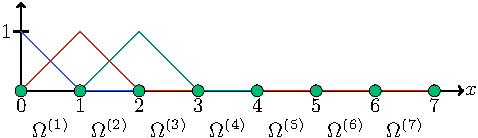
\includegraphics[width=0.6\textwidth]{pics/1dDomain}
\caption{A discretized 1D domain with nodes in green and linear ansatz functions shown for the first four nodes}
\label{fig:1DDom}

\end{center}
\end{figure}
%
\begin{figure}[h]
\begin{center}

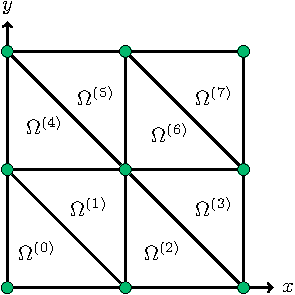
\includegraphics[width=0.4\textwidth]{pics/2dDomain}
\caption{A discretized 2D domain with nodes in green}
\label{fig:2DDom}

\end{center}
\end{figure}
%
The finer the mesh, i.e. the more elements are used in a domain, the closer the FEM approximation comes to the exact solution. Since computing very fine meshes is computationally expensive, a convergence study is conducted in order to find the element size from which on smaller element sizes don't result in more accurate results.

Using FEniCS, a 1D mesh can be created by calling
\begin{minted}
[
frame=lines,
framesep=2mm,
baselinestretch=1.2,
bgcolor=backcolour,
fontsize=\footnotesize,
linenos
]
{python}
self.dom_a = 0.0 #domain boundaries
self.dom_b = 1.0
self.ne	= 60 #number of elements
self.mesh = IntervalMesh(self.ne,self.dom_a,self.dom_b) #define mesh
\end{minted}
The interval of the mesh and the desired number of elements have to be provided.

A 2D mesh can, for example, be obtained by calling
\begin{minted}
[
frame=lines,
framesep=2mm,
baselinestretch=1.2,
bgcolor=backcolour,
fontsize=\footnotesize,
linenos
]
{python}
self.a,self.b = 2,2
self.mesh = UnitSquareMesh(self.a,self.b) #define mesh
\end{minted}
In this case a unit square is chosen what means that the domain size will be quadratic and of length $1.0$ in every direction. $2$ elements were chosen for every dimension what leads to a mesh looking like \ref{fig:2DDom}. Of course every desired 2D shape can be used as a mesh.

\subsection{Approximation and Building Element Matrices}
In the FEM, the values between nodes within an element are interpolated with basis functions $\varphi_i$. 
For each node in the domain an FEM basis function is defined. By weighing those basis functions, the solution can be approximated with 
\begin{equation}
p(x_i) = \sum_{j \in \Omega} c_j  \varphi_j(x_i) = f(x_i) \; .
\label{eqn:WeighingFunction}
\end{equation}
(\ref{eqn:WeighingFunction}) means, that the value of one particular point $x_i$ is the sum of all products of all weight coefficients $c_j$ and test functions $\varphi_j$ evaluated at that point. If now orthogonal basis functions are used, as it is commonly the case in FEM, (\ref{eqn:WeighingFunction}) simplifies as described below. One popular choice of orthogonal basis functions is the Lagrange family of polynomials. The right hand side $f(x_i)$ does, in practice, describe the source term of the PDE which does not depend on $p(x)$.

\paragraph{Lagrange Polynomials}
[Langtangen FEM]
Lagrange polynomials are one possible choice for FEM basis functions and are used in this thesis. They can be calculated for any desired degree $N$ and their main property is that they are orthogonal to one another. They are used as an interpolation between given points which means that they polynommial always exactly gows through the given points. The behaviour at all other points is determined by the definition of the Lagrange polynomial
\begin{equation}
\varphi_i(x) = \prod_{j=0,j\neq i}^N \frac{x-x_j}{x_i-x_j} \;.
\end{equation}
They are frequently used in FEM because there holds 
\begin{equation}
\varphi_i(x_s) = \delta_{is}, \quad \delta_{is}  =     \left\{ \begin{array}{rcl} 1 & \mbox{for}& i = s  \\ 0 & \mbox{for} & i \neq s\end{array}\right .
\end{equation}
which means that the polynomial is only $1$ at one node in the domain. At all other nodes it is $0$. Between nodes the Lagrange polynomial is spanned. This behavior simplifies (\ref{eqn:WeighingFunction}):
\begin{equation}
p(x_i) = c_i \varphi_i(x_i) = c_i \;.
\end{equation}
The weight factor is therefore the true value at the node.
Another asset of using orthogonal polynomials is that $\varphi_i(x)$ is $0$ in most parts of the domain what leads to diagonal matrices which can be solved much quicker than densely packed ones.
%
The goal is to solve the linear system of equations for the weight factors $c_i$ and therefore $p(x)$. It can be notated as
\begin{equation}
\sum_j A_{i,j} c_j = b_i
\end{equation}
with
\begin{align}
A_{i,j} &= \varphi_j(x_i), \\
b_i &= f(x_i) \;.
\end{align}
The calculation is usually done for one element at a time. Therby arises an element matrix $A^{(e)}$ whose individual entries can be computed as
\begin{equation}
A_{r,s}^{(e)} = \int_{\Omega^{(e)}} \varphi_r \varphi_s \, \mathrm{d}x 
\end{equation}
with $i,j$ the numbers of the individual nodes in an element. For linear elements, i.e. elements with two nodes each, a $2\times 2$ matrix results and for quadratic elements with three nodes each a $3\times3$ matrix results.

Also the right hand side vector $b$ is computed element-wise:
\begin{equation}
b_r^{(e)} = \int_{\Omega^{(e)}} f(x) \varphi_r \, \mathrm{d}x \; .
\end{equation}


\subsection{Assembling and Solving the System}

The element matrices are then assembled to a global system matrix. Within an element, the coordinates of the nodes are $[0,...,d]$ with $d$ the dimension of the element. For linear elements, the coordinates are $[0,1]$. For assembly they need to be mapped to the global coordinate system. This is accomplished by using a mapping function, noted as $q$ which maps $[r,s]$ of the elements to $[i,j]$ in the global system: $i=q(e,r)$ and $j = q(e,s)$ with $e$ the number of the element. For the global system matrix there now holds
\begin{equation}
A_{q(e,r), q(e,s)} := A_{q(e,r), q(e,s)} + A_{r,s}^{(e)}
\end{equation}
through which can be iterated using a loop in Python. 
The resulting matrix is sparse, here for three elements with linear ansatz functions:
\begin{equation}
A_{q(e,r), q(e,s)}  =
\begin{bmatrix}
\textcolor[rgb]{0.49,0.83,0.13}{A_{0,0}^{( 0)}} & \textcolor[rgb]{0.49,0.83,0.13}{A}\textcolor[rgb]{0.49,0.83,0.13}{_{0,1}^{( 0)}} & 0 & 0\\
\textcolor[rgb]{0.49,0.83,0.13}{A}\textcolor[rgb]{0.49,0.83,0.13}{_{1,0}^{( 0)}} & \textcolor[rgb]{0.49,0.83,0.13}{A}\textcolor[rgb]{0.49,0.83,0.13}{_{1,1}^{( 0)}}\textcolor[rgb]{0,0,0}{+}\textcolor[rgb]{0.49,0.83,0.13}{\ }\textcolor[rgb]{0.82,0.01,0.11}{A_{0,0}^{( 1)}} & \textcolor[rgb]{0.82,0.01,0.11}{A}\textcolor[rgb]{0.82,0.01,0.11}{_{0,1}^{( 1)}} & 0\\
0 & \textcolor[rgb]{0.82,0.01,0.11}{A}\textcolor[rgb]{0.82,0.01,0.11}{_{1,0}^{( 1)}} & \textcolor[rgb]{0.82,0.01,0.11}{A}\textcolor[rgb]{0.82,0.01,0.11}{_{1,1}^{( 1)} \ }\textcolor[rgb]{0,0,0}{+}\textcolor[rgb]{0.29,0.56,0.89}{A_{0,0}^{( 2)}} & \textcolor[rgb]{0.29,0.56,0.89}{A}\textcolor[rgb]{0.29,0.56,0.89}{_{0,1}^{( 2)}}\\
0 & 0 & \textcolor[rgb]{0.29,0.56,0.89}{A}\textcolor[rgb]{0.29,0.56,0.89}{_{1,0}^{( 2)}} & \textcolor[rgb]{0.29,0.56,0.89}{A}\textcolor[rgb]{0.29,0.56,0.89}{_{1,1}^{( 2)}}
\end{bmatrix} \ \ 
\end{equation}


For the global right-hand-side vector there holds
\begin{equation}
b_{q(e,r)} := b_{q(e,r)} + b_r^{(e)} \; .
\end{equation}
With FEniCS, the system is assembled by 
\begin{minted}
[
frame=lines,
framesep=2mm,
baselinestretch=1.2,
bgcolor=backcolour,
fontsize=\footnotesize,
linenos
]
{python}
A = assemble(a)
b = assemble(L)
\end{minted}
The system of equations can now be solved for the vector of unknowns by calling
\begin{minted}
[
frame=lines,
framesep=2mm,
baselinestretch=1.2,
bgcolor=backcolour,
fontsize=\footnotesize,
linenos
]
{python}
self.u = Function(self.V) 
U = self.u.vector()
solve(A, U, b)
\end{minted}

\subsection{Setting Constraints}


\subsection{Solving and Convergence}
explain how the linear system is solved (LU decomp or Cholesky)







\chapter{Gaussian Processes and the Statistical Finite Element Method}

\section{Basic Probability Theory}
The statistical Finite Element Method (statFEM) is based on Gaussian Processes (GPs) and Bayesian inference. To be able to work with both, some basic understanding of probability theory is necessary.

\subsection{Gaussian Distribution}
speak about linearity somewhere! see Römer lectures

explain PDF/CDF and moments

explain the multivariate gaussian

A random variable $X$ is considered normally, or Gaussian, distributed if $X \sim \mathcal{N}(\mu, \sigma)$ with $\mu$ the mean and $\sigma$ the standard deviation. The shape of the PDF is a bell curve.

From any distribution, the moments of the random variable can be deduced. Using the PDF there holds for the mean
\begin{equation}
\mu = \mathbb{E}[X] = \int_{\mathbb{R}} x f_X(x) \, \mathrm{d}x
\end{equation}
%
and for the variance
\begin{equation}
\mathbb{V}[X] = \mathbb{E}[(X-\mathbb{E}[X])^2] = \mathbb{E}[X^2] - \mathbb{E}[X]^2 \;.
\end{equation}

For the PDF of the Gaussian distribution there holds
\begin{equation}
f_X(x) = \frac{1}{\sigma \sqrt{2 \pi}} \exp(-\frac{1}{2} \left(\frac{x-\mu}{\sigma}\right)^2)
\end{equation}

If multiple random variables are observed, which are all normally distributed, they can be aggregated in a so-called multivariate Gaussian disribution. Instead of a random variable it is a random vector which is defined by a mean vector and a covariance matrix. The matrix is named covariance and not variance matrix because not only the variance of the individual random variables but also the covariance among the different variables makes up entries of it. It is simlar to auto- and cross correlation, both described in a single matrix.
For the PDF of a multivariate Gaussian distribution there holds
\begin{equation}
f_X(\bm{x}) = \frac{\exp(-\frac{1}{2}(\bm{x}-\bm{\mu})^T \Sigma^{-1}(\bm{x}-\bm{\mu}))}{\sqrt{(2\pi)^k \lvert \Sigma \rvert}}
\end{equation}
with $\Sigma$ the covariance matrix, $\bm{\mu}$ the mean vector and $k$ the dimension, i.e. the number of random variables, of the distribution.
An example of a multivariate Gaussian is visible in Figure \ref{fig:MultiGauss}. The underlying mean vector and covariance matrix read
\begin{equation}
\bm{\mu} = \begin{bmatrix}
           0 \\
           1
         \end{bmatrix}
, \quad     
\Sigma = \begin{bmatrix}
1 & -0.7 \\
-0.7 & 1.5 
\end{bmatrix} \;.
\end{equation}
The smaller the absolute of the non-diagonal entries of the covariance matrix is, the less correlated the individual variables are.

\begin{figure}[h]
\begin{center}
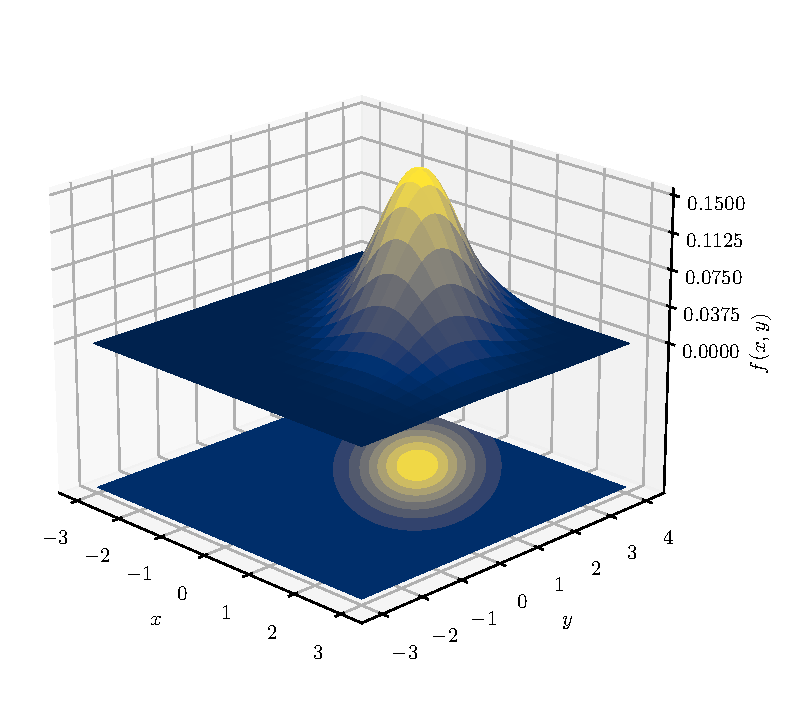
\includegraphics[width=0.6\textwidth]{pics/Gaussians}
\caption{A multivariate Gaussian distribution with two dimensions. A strong correlation between the two random variables is visible. [scipy tutorial] }
\label{fig:MultiGauss}
\end{center}
\end{figure}

\subsection{Bayesian Inference}
$posterior = \frac{likelihood x prior}{marginal likelihood}$ (Rasmussen p.9)
explain basics of bayesian inference with bayes rule etc. what is posterior/prior 
explain what the marginal likelihood is

\paragraph{Marginal Likelihood}


\section{Gaussian Process Regression}

\subsection{Regression}
"Regression is used to find a function that rerpesents a set of data points as closely as possible" [Visual Exploration]
[Visual Exploration] "A Gaussian process is a probabilistic method that gives confidence for the predicted function"

"GPs allow us to make predictions about our data incorporating prior knowledge"



The following closely follows [Rasmussen].


Gaussian Processes are a class of Bayesian non-parametric models. Non-parametric doesn't mean that there are no parameters involved but rather that there is an infinite number of them. Every realization of a Gaussian process doesn't yield a scalar or vector but a function. One can think of a Gaussian Process as a collection of infinitely many normally distributed random variables, i.e. a generalization of a Gaussian distribution: A vector with infinitely many entries is basically a function. By picking out a finite set of those random variables when discretizing e.g. on an FEM mesh, one obtains a multivariate distribution which is determined by a mean and a covariance matrix. [Rasmussen p.2] Hence, the GP assigns a confidence band to a function where a usual parametric regression wouldn't.

A GP is described by its mean function and the covariance function, also called kernel.

\subsection{Marginalization and Conditioning} 
Marginalisation means that out of a multivariate Gaussian the single variables can directly be taken out of the mean vector and the covariance matrix. E.g. for a point on the axis describved by the GP, a single value can be picked out. A univariate Gaussian comes out by simply using the mean vectors value at that point and the i,i th index of the covariance matrix. This means that the underlying distributions for single variables do not change if a GP is used to describe an arbitrary set of variables [p13].
[Visual Exploration]
From a multivariate, in this case bivariate, Gaussian
\begin{equation}
P(X,Y) = \begin{bmatrix}
           X \\
           Y
         \end{bmatrix} \sim \mathcal{N}\left( \begin{bmatrix}
           \mu_X \\
           \mu_Y
         \end{bmatrix}, \begin{bmatrix}
\Sigma_{XX} & \Sigma_{XY} \\
\Sigma_{YX} & \Sigma_{YY} 
\end{bmatrix}  \right)
\end{equation}
one single random variable, say $X$, can be marginalized out by simply only looking at the entries corresponding solely to $X$:
\begin{equation}
X \sim \mathcal{N}(\mu_X, \Sigma_{XX}) \;.
\end{equation}
If the covariance matrix and mean vector are not known, a random variable can be marginaluzed out of an arbitrary distribution by
\begin{equation}
p_X(x) = \int_y p_{X,Y}(x,y)\,\mathrm{d}y = \int_y p_{X|Y}(x|y)p_Y(y)\,\mathrm{d}y
\label{eqn:margi}
\end{equation}
which intuitively means that summing the probability for $X$ at every possible $Y$ gives the total probability for $X$ independent of $Y$. 

(\ref{eqn:margi}) already uses the principle of conditioning. The condition operator $|$ yields the probability of one variable under the condition that another variable is true. As an illustration in words one could ask: "What is the probability of event $X$ to happen under the condition, that the event $Y=y$ happens simultaneously?"
For the mutlivariate Gaussian there holds for the conditioning
\begin{equation}
X|Y \sim \mathcal{N}(\mu_X +\Sigma_{XY} \Sigma_{YY}^{-1}(Y-\mu_Y), \Sigma_{XX} - \Sigma_{XY}\Sigma_{YY}^{-1}\Sigma_{YX} ) \;.
\end{equation}
%
Conditioning yields a so-called modified Gaussian distribution which can be imagined as a "cut" through a multivariate Gaussian $P(X,Y)$ at a certain point $y$. A new Gaussian with the dimension reduced by $1$ arises as illustrated in Figure \ref{fig:GaussCut3d}.

%
%
\begin{figure}[h]
\begin{center}
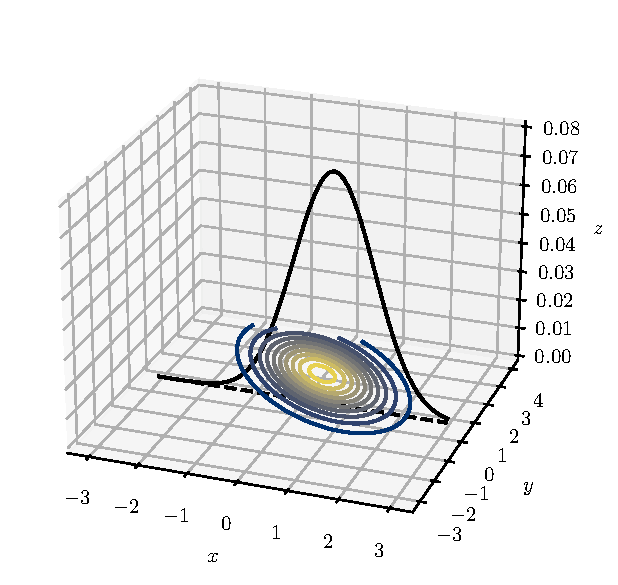
\includegraphics[width=0.6\textwidth]{pics/Gaussians3dCut}
\caption{Cutting, i.e. conditioning, a bivariate Gaussian at the dashed line leads to a new Gaussian with only one dimension.}
\label{fig:GaussCut3d}
\end{center}
\end{figure}



-Regression in general
-differences of a GP regression to e.g. a polynomial regression: every point is assgined an uncertainty

-a distribution over functions

-Herleitung der Kovarianzmatrix, evtl. auch für das standard linear regression modell

-parameter variations

\subsection{Gaussian Processes}


\subsection{Kernel Functions}
p14:

If a kernel function is evaluated at a finite number of points, one gets a covariance matrix. This can be used as the covariance of a Gaussian vector from which samples can be drawn. The values of each entry are a function over the input points of the kernel function.

p79: in a covariance function all the assumptions of the function to be modeled are contained. The kernel defines or rather assesses how near or similar a value of one point is to the one of another. A training point which is close to a test point therefore gives information on how the value at the test point should be.

\paragraph{Stationary Kernels} are a function of $x-x'$. They are stationary because it doesn't matter what value $x$ and $x_prime$ have as a starting value, the difference is always the same. Example: $1100mm -1000mm = 100 mm, 100100mm-100000mm = 100mm$


p80: A radial basis function is a function which is !only! a function of $r=x-x'$ and whioch is therefore isotropic, i.e. there are no rigid motions. r is like a radius so these functions are called radial basis functions.

Covariance matrices always have to be symmetric, i.e. $k(x-x') = k(x'-x)$, since everything else wouldnt make sense

The so-called Gram matrix is the function containing $x-x'$ evaluated at a set of points $x_i$. if the function is a covariance funtion, the gram matrix is called covariance matrix.
\paragraph{The Squared Exponential Kernel Function} is the most commonly used kernel function for GPs. It is stationary and infinitely differentiable, hence very smooth. 
It is defined as
\begin{equation}
k_{SE} = \sigma \exp(-\frac{r^2}{2l^2})
\end{equation}
%
and can be defined as a Python function with
[Code von Murphy] 
\begin{python}
def squared_exponential(xa, xb, l, sig):
    sq_norm = -0.5 * scipy.spatial.distance.cdist(xa, xb, 'sqeuclidean') \
    	* (1/l**2)
    return sig**2 * np.exp(sq_norm) .
\end{python}
\label{lst:sqEx}


\begin{figure}[h]
\begin{center}

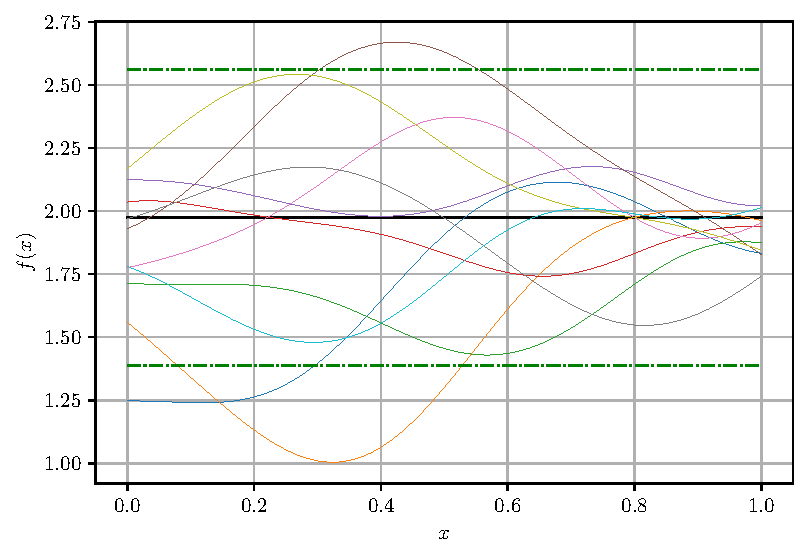
\includegraphics[width=0.6\textwidth]{pics/sqexp_f_sampled}
\caption{The source term GP of $f(x)$ sampled for a Squared Exponential kernel with $l = 0.25$ and $\sigma = 0.3$. $\bar{f}(x)$ in solid black, $2\sigma$ confidence bands in green.}
\label{fig:Matern1_2}

\end{center}
\end{figure}

\paragraph{Positive Definiteness}A covariance function has to be positive semidefinite, i.e. all eigenvalues are greater or equal zero. A covariance matrix K is positive semidefinite when $Q(v) = v^T K v \geq 0$. Q is the quadratic form. A kernel function is positive semidefinite if it only outputs matrices which are positive semidefinite.


\paragraph{The Characteristic Length Scale} can be thought of as the number of "upcrossings" in the interval, i.e. the number of crossings of the x axis. It can be calculated with eq 4.3. rasmussen. The more upcrossings, the shorter the length scale.

\paragraph{Matern Kernel Functions}
[Rasmussen] The squared exponential kernel is infinitely differentiable, which means that it behaves very smoothly. This is considered as unphysical by [Stein]. Therefore, the Matern class of covariance functions is recommended which is finitely differentiable and therefore less smooth. It is called a "class" of kernels because by varying the parameters, very different behaviours can be obtained. The squared exponential kernel is actually a special case of the Matern class.

The general Matern kernel is defined as
\begin{equation}
k_M(r) = \sigma^2 \frac{2^{1-\nu}}{\Gamma(\nu)}  \left( \frac{\sqrt{2\nu}r}{l}  \right)^{\nu} K_{\nu}  \left(  \frac{\sqrt{2\nu}r}{l}   \right)
\label{eqn:MaternKernel}
\end{equation}
with $\Gamma(\nu) = (\nu - 1)!$ the gamma function and $K_{\nu}$ a modified Bessel function [Abramowitz Stegun] [Rasmussen]. $\nu$ and $l$ are free positive parameters.
For $\nu \to \infty$  (\ref{eqn:MaternKernel}) becomes the squared exponential kernel.
The covariance function simplifies for half integer values of $\nu$ and can be expressed as a product of an exponential and a polynomial. According to [Rassmussen] $\nu = 3/2$ and $\nu = 5/2$ are commonly used for GPs; the simplest Matern kernel is obtained with $\nu = 1/2$:

\begin{align}
k_{M;\nu = 1/2}(r) &=   \sigma^2 \exp(- \frac{r}{l})  \; , \\
\label{eqn:Materns1}
k_{M;\nu = 3/2}(r) &=  \sigma^2 \left(      1+ \frac{\sqrt{3}r}{l}  	\right)  \exp(- \frac{\sqrt{3} r}{l})  \; , \\
k_{M;\nu = 5/2}(r) &=  \sigma^2\left(      1+ \frac{\sqrt{5}r}{l}  + \frac{5r^2}{3l^2}	\right)  \exp(- \frac{\sqrt{5} r}{l}) \; .
\label{eqn:Materns3}
\end{align}
%
(\ref{eqn:Materns1}) - (\ref{eqn:Materns3}) are used in this thesis. Figures \ref{fig:Matern1_2} - \ref{fig:Matern5_2} show the differences between the different choices for $\nu$: The higher it is chosen, the smoother the GP becomes and the closer it gets to the squared exponential kernel.
\begin{figure}[h]
\begin{center}

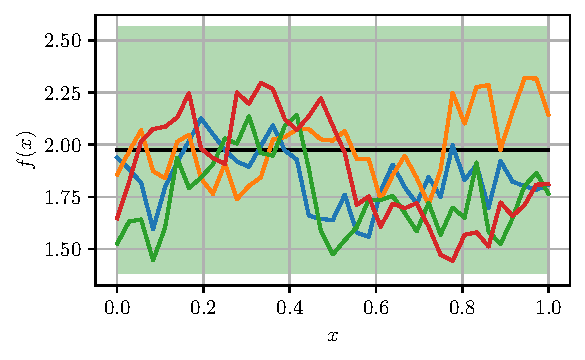
\includegraphics[width=0.6\textwidth]{pics/matern1_2_f_sampled}
\caption{The source term GP of $f(x)$ sampled for a Matern kernel with $\nu=1/2$. $\bar{f}(x)$ in solid black, $2\sigma$ confidence bands in green.}
\label{fig:Matern1_2}

\end{center}
\end{figure}

\begin{figure}[h]
\begin{center}

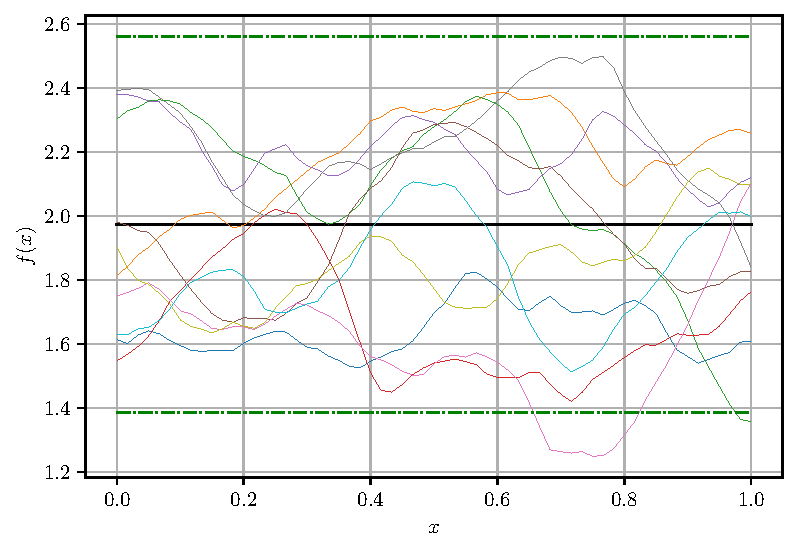
\includegraphics[width=0.6\textwidth]{pics/matern3_2_f_sampled}
\caption{The source term GP of $f(x)$ sampled for a Matern kernel with $\nu=3/2$. $\bar{f}(x)$ in solid black, $2\sigma$ confidence bands in green.}
\label{fig:Matern3_2}

\end{center}
\end{figure}

\begin{figure}[h]
\begin{center}

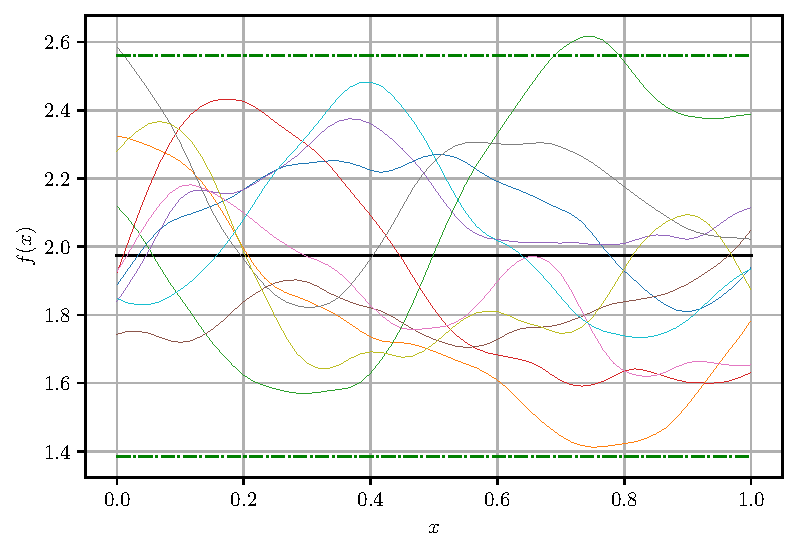
\includegraphics[width=0.6\textwidth]{pics/matern5_2_f_sampled}
\caption{The source term GP of $f(x)$ sampled for a Matern kernel with $\nu=5/2$. $\bar{f}(x)$ in solid black, $2\sigma$ confidence bands in green.}
\label{fig:Matern5_2}

\end{center}
\end{figure}


\paragraph{Periodic Kernel Functions}

\paragraph{Combination of Different Kernel Functions}


hyperparameters

hyperparameter learning

marginal likelihood: integral of the likelihood times the prior
marginal means marginalization over the function values so these dont appear in the equation anymore. in this case it's marginalizing over the test points X so those dont appear anymore.


\subsection{Prior before observation}
explain, how a sample from the multivariate gaussian canbe drawn (A2 Rasmussen).
To obtain a sample from the mutlivariate Gaussian which represents the GP, at first the Cholesky decomposition of the covariance matrix $\Sigma = LL^T$ has to be computed. Next, a sample from a standard multivariate normal distribution $\bm{u} \sim \mathcal{N} (\bm{0},\bm{I})$ is drawn. The final sample $\bm{x}$ can now be obtained using
\begin{equation}
\bm{x} = \bm{m} + L \bm{u} 
\end{equation}
with the prescribed mean vector $\bm{m}$.
With Python and numpy, the sample is obtained with
\begin{minted}
[
frame=lines,
framesep=2mm,
baselinestretch=1.2,
bgcolor=backcolour,
fontsize=\footnotesize,
linenos
]
{python}
x = np.random.multivariate_normal(
			mean = mean, cov=Sig,
			size=1)
\end{minted}			
The numpy function does the Cholesky decomposition internally.
	
	
			
\paragraph{Occam's Razor}

\subsection{Posterior after observation}
p16:
The prior is conditioned on the observations. It would also be possible, abut computationally demanding, to sample many many functions out of the GP and only take those which go through the training points.

explain conditioning



\section{The Statistical Finite Element Method}
The FEM is based on a model in form of a differential equation which is used to describe some kind of phenomenon, in the case of this thesis vibroacoustics, as accurately as possible. However, every model is only an approximation of reality which gives rise to a model inadequacy error: There is some unknown physics hidden between the model and reality. By collecting data, basically measuring reality with some kind of measurement error, that discrepancy $d$ between model and reality can be infered. That is what statFEM aims to do: It finds a new model, based on data, which solves the model inadequacy of the FEM.

\paragraph{The Statistical Generating Model}
Measuring data always involves a measurement error: One can never measure any physical quantity without some measurement noise. Therefore, the so-called statistical generating model (Cirak) for a vector of $n_y$ measurements $\bm{y} \in \mathbb{R}^{n_y}$, 
%
\begin{equation}
\bm{y} = \bm{z} + \bm{e} = \rho \bm{P} \bm{u} + \bm{d} + \bm{e} \; ,
\end{equation}
%
consists of response of the true underlying process $\bm{z} \in \mathbb{R}^{n_y}$ at the measurement points and the measurement noise $\bm{e} \in \mathbb{R}^{n_y}$. The true process $\bm{z}$ can further be expressed as a combination of the used model $\bm{u} \in \mathbb{R}^{n_u}$, which tries to describe the true process, and a model discrepancy error $d$ which accounts for the model not being a completely accurate representation of the true physics. The model is scaled using the scaling parameter $\rho \in \mathbb{R}$. It can be evaluated at $n_u$ points which are determined by the FEM mesh but only its evaluations at the measurement points are taken into account by using the projection matrix $\bm{P} \in \mathbb{R}^{n_y \times n_u}$.
%
$e$ is modeled as a multivariate Gaussian 
%
\begin{equation}
\bm{e} \sim p(\bm{e}) = \mathcal{N}(\bm{0}, \bm{C_e})
\end{equation}
with zero mean and the covariance matrix $\bm{C_e} = \sigma_e^2 \bm{I}$ which adds the measurement noise to each entry of $\bm{z}$.
%
The model discrepancy error is, in order to account for a possibly complex behavior, modeled as a GP
\begin{equation}
\bm{d} \sim p(\bm{d} | \sigma_d, l_d) = \mathcal{N}(\bm{0},\bm{C_d})
\end{equation}
which $\sigma_d, l_d$ the unknown parameters of a squared exponential kernel function. Evaluating it at the measurement positions, the GP is represented by a multivariate Gaussian with a covariance matrix $\bm{C_d} \in \mathbb{R}^{n_y \times n_y}$.




\paragraph{Basic statFEM procedure}
statFEM can basically be broken down into three major steps[Cirak, abstract]. The first one is applying Bayesian inversion to the FEM part of the solution. The prior GP is constructed and evaluated before data is introduced. Equations are derived which incorporate the data in order to compute a posterior density for the FEM solution GP. The equations for that solution are dependent on certain hyperparameters. These are estimated in the second step: For each of the hyperparameters a posterior density is calculated using a prior and the marginal likelihood. The third and last step is in principle finding a proper mesh size which is able to describe data the best. This last step may appear rather unimportant since usually in FEM the consensus is that a finer mesh leads to a more accurate result. However, it will be demonstrated that the optimum element size strongly depends on the value of certain hyperparameters estimated in step 2 and that there is a correlation between relatively inaccurate statFEM results and a too small element size.

\subsection{Step 1: Posterior of the FEM Forward Model}

\paragraph{Assembling the FEM System Matrix}
The FEM assembly and solving is handled by Fenics. To compute the system matrix and to later solve for the vector of unknowns, the PDE has to be defined in a variational formulation as a boundary value problem.
At first, the FEM solver is initiated by defining the domain, the wished number of elements and the kind of elements to be used. In this example, a 1 dimensional mesh with Lagrange basis functions is used.
\begin{python}
def __init__(self, nMC = 200):
	self.dom_a = 0.0 #domain boundaries
	self.dom_b = 1.0
	self.ne	= 100 #number of elements
	self.mesh = IntervalMesh(self.ne,self.dom_a,self.dom_b) #define mesh
	self.bbt = self.mesh.bounding_box_tree()
	self.coordinates = self.mesh.coordinates() # vertices vector
	self.V = FunctionSpace(self.mesh, "Lagrange", 1) # Function space
\end{python}
The variational formulation for the chosen PDE consists of a linear form $L$ and a bilinear form $a$. These need to be specified individually for Fenics. The boundary condition is set to $u_0 = 0.0$ for both boundaries in the 1D mesh. The system matrix $A$ can be returned by calling \mintinline{python}{A = assemble(a)}. The boundary conditions are applied to $A$ after assambly.

\begin{minted}
[
frame=lines,
framesep=2mm,
baselinestretch=1.2,
bgcolor=backcolour,
fontsize=\footnotesize,
linenos
]
{python}
def doFEM(self):
	# Define Dirichlet boundary (x = 0 or x = 1)
	def boundary(x):
		return x[0] < (self.dom_a + DOLFIN_EPS) or x[0] > self.dom_b - DOLFIN_EPS
	# Define boundary condition
	u0 = Constant(0.0)
	self.bc = DirichletBC(self.V, u0, boundary)
	# Define variational problem
	self.u = TrialFunction(self.V)
	self.v = TestFunction(self.V)
	# find index of cell which contains point.
	class DoGP(UserExpression):
		def eval(self, value, x):
			collisions1st = bbt.compute_first_entity_collision(Point(x[0])) 
			value[0] = f_vals[collisions1st] # f is constant in a cell.
		def value_shape(self):
			return ()
	f_vals = self.draw_FEM_samples(coordinates)
	f_vals = f_vals[0]
	f = DoGP()
	
	a = dot(grad(self.u), grad(self.v))*dx #variational Problem
	L = f*self.v*dx

	A = assemble(a)
	b = assemble(L)
	self.bc.apply(A, b)
	
	U = self.u.vector()
	solve(A, U, b)
	return U, A

\end{minted}


\paragraph{Generate and Sample From Source Term GP}
The differential equation is treated from a Bayesian viewpoint: all parameters are random variables. For dependent parameters, such as a source term $f(x)$ dependent on the spatial coordinate, not a single distribution but a Gaussian Process is applied. Therefore prior to solving the FEM linear system, the parameter $ \mathcal{GP} ( \bar{f},C_f)$ is sampled. That sample is evaluated for each cell in the FEM mesh which makes it necessary to assemble the system matrix with that in mind. 
$\bar{f}$ is set to a prescribed value. $C_f$ is calculated using the prescribed hyperparameters of the chosen kernel function. As an example, a sample from $ \mathcal{GP} ( \bar{f},C_f)$ can be drawn for a Matern kernel by calling
\begin{minted}
[
frame=lines,
framesep=2mm,
baselinestretch=1.2,
bgcolor=backcolour,
fontsize=\footnotesize,
linenos
]
{python}
def sample_f(self):
	c_f = self.matern_log(self.coordinates,
		self.coordinates, l=np.log(lf), sig=np.log(sigf))
	f_mean = (np.pi)**2*(1/5)*np.ones(self.ne+1)
	fGP = np.random.multivariate_normal(
		mean = f_mean, cov=c_f,
		size=10)
\end{minted}
Here, the Matern kernel accepts only the $\log$ of the parameters $lf$ and $sigf$.

\paragraph{Generate and sample from the diffusion coefficient GP}
If the diffusion coefficient $\kappa$ is assumed to be a random variable and dependent on $x$, it can be modeled as a GP as well and there holds
\begin{equation}
\kappa \sim \mathcal{GP}(\bar{\kappa},C_{\kappa})
\end{equation}

\paragraph{Computing the FEM Prior}
Having the GPs for the input parameters defined, the FEM system of equations can be solved. With the input parameters defined as a GP, also the FEM solution is going to be a GP. Therefore, 
\begin{equation}
u \sim \mathcal{GP}(\bar{u}, C_u)
\end{equation}
is to be calculated. Expressed in terms of the FEM system matrix, there holds
\begin{equation}
\bm{u} = \bm{A}^{-1}\bm{f}
\end{equation}
Because of discretizing, the multivariate Gaussian
\begin{equation}
\bm{u} \sim p(u) = \mathcal{N} \left( A^{-1} \bar{f}, A^{-1} C_f A^{-T}  \right)
\label{eqn:u_GP_disc}
\end{equation}
arises.
As visible in (\ref{eqn:u_GP_disc}), there holds for $\bar{u}$
\begin{equation}
\bar{u} = A^{-1} \bar{f} \; ,
\end{equation}
which can be computed using Python by calling
\begin{python}
def get_U_mean(self):
	u_mean = Function(self.V)
	U_mean = u_mean.vector()
	b_mean = assemble(f_mean*self.v*dx) 
	self.bc.apply(b_mean)
	solstd,A = self.doFEM()  # solstd is unused here.
	solve(A,U_mean,b_mean)
	return U_mean .
\end{python}
\label{lst:get_u_mean}
$C_u$ is obtained by calculating
\begin{equation}
A^{-1} C_f A^{-T} \; .
\end{equation}
In Python code there holds
\begin{python}
def get_C_u(self):
	C_f = self.get_C_f()
	solstd,A = self.doFEM()
	ident = np.identity(len(self.coordinates))
	self.bc.apply(A)
	A = A.array()
	A_inv = np.linalg.solve(A,ident)
	thresh = 1e-16
	C_u = np.dot( np.dot(A_inv,C_f), np.transpose(A_inv))
	C_u = C_u + 1e-16*(self.sigf**2)*ident
	c_u = np.transpose(self.integratedTestF) * C_u * self.integratedTestF
	return C_u .
\end{python}
\label{lst:get_C_u}
With $\bar{u}$ and $C_u$ the GP for the prior is completely defined. 
\paragraph{Find Prior Mean and Variance}
Once the prior is computed, it can be sampled. The mean is already given but the parameters of the underlying GP are unknown. It is possible to evaluate $C_u$ for the standard deviation with
\begin{equation}
\bm{\sigma_u} =  \mathrm{diag}(C_u)
\label{eqn:varCu}
\end{equation}
In Python
\begin{minted}
[
frame=lines,
framesep=2mm,
baselinestretch=1.2,
bgcolor=backcolour,
fontsize=\footnotesize,
linenos
]
{python}
C_u_sig = np.sqrt(np.diagonal(C_u))
\end{minted}
solves (\ref{eqn:varCu}).

\paragraph{The Projection Matrix $P$}
The projection matrix $P$ is constructed by evaluating all FEM ansatz functions of the mesh at the $n_y$ measurement positions. The result is a sparse matrix with most entries zero and only those entries non zero that correspond to the ansatz functions $\Phi_i(\bm{\bm{x}})$ associated with the finite element in which the measurement positions lie.
This computation for linear ansatz functions can easily be implemented in Python using Fenics:

\begin{python}
def getP(self,y_points):
	ny = len(y_points)
	P = np.zeros((ny, self.ne+1), dtype = float) #with ne the number of elements
	for j,point in enumerate(y_points):
		x = np.array([point])
		x_point = Point(x)
		bbt = self.mesh.bounding_box_tree()
		cell_id = bbt.compute_first_entity_collision(x_point)
		cell = Cell(self.mesh, cell_id)
		coordinate_dofs = cell.get_vertex_coordinates()
		values = np.ones(1, dtype=float)
		for i in range(self.el.space_dimension()): 
			phi_x = self.el.evaluate_basis(np.array(i),x 
				,np.array(coordinate_dofs),cell.orientation())
			P[j,cell_id+i] = phi_x
	self.Pu = np.dot(P,self.U_mean)
	return P
\end{python}
\label{lst:getP}
\paragraph{Calculate $C_e$}
$C_e$ is the measurement error term. It is defined in Python by
\begin{minted}
[
frame=lines,
framesep=2mm,
baselinestretch=1.2,
bgcolor=backcolour,
fontsize=\footnotesize,
linenos
]
{python}
def get_C_e(self,size):
	sige_square = 2.5e-5
	C_e = sige_square * np.identity(size)
	return C_e
\end{minted}

\paragraph{Calculate $C_d$}
The model discrepancy term $C_d$ is modeled as a GP with mean $\bar{d} = 0$. Therefore it can be obtained by calling
\begin{minted}
[
frame=lines,
framesep=2mm,
baselinestretch=1.2,
bgcolor=backcolour,
fontsize=\footnotesize,
linenos
]
{python}
def get_C_d(self,y_points,ld, sigd):
	C_d = self.matern_log(y_points, y_points, l=ld, sig=sigd)
	return C_d
\end{minted}
The points in the domain and the hyperparameters have to be provided in order to calculate the covariance function. The latter ones are not yet known and need to be estimated, see below for a thorough explanation on that.

\subsection{Inference of the Posterior Density}
To infer the posterior density, observed data is necessary. These can be obtained by either actually measuring a physical process or by generating synthetic data which allows developing and improving the statFEM model already before having to set up an experiment and take real measurements beforehand.
%
Sampling from a synthetic source or from the real physical response yields the observation vector
%
\begin{equation}
\bm{y} = {z} + {e}
\end{equation}
%
with $z$ the real response and $e$ the measurement error which is also a part of $\bm{y}$ for the synthetic observations. It can be seen that the model mismatch error $\bm{d}$ is, as opposed to eq. (), not part of the equation because it is only part of the FEM modeling error. 
%
The data is observed on multiple measurement  points $n_y$ throughout the domain. It can be chosen if the data is assumed to be deterministic or to be random. For the deterministic case only one value is measured for each measurement point. In the random case many measurements are taken per point what leads to a probability distribution for each point.
%
Now, Bayes' rule can be applied to update the prior with the observations.
The result of this operation is
%
\begin{equation}
p(u|y) = \mathcal{N}(\bar{u_{|y}}, C_{u|y})
\end{equation}
%
with
%
\begin{equation}
\bar{u_{|y}} = C_{u|y} \left(   \rho P^T  (C_d + C_e)^{-1}  y  +  C_u^{-1}  \bar{u}   \right)
\end{equation}
and
\begin{equation}
C_{u|y} = \left(      \rho^2  P^T   (C_d + C_e)^{-1}  P  +  C_u^{-1}    \right)^{-1}
\end{equation}


\subsection{find Posterior mean and variance}


\subsection{Modeling Parameters of the PDE}

\subsection{Probabilistic FEM Prior}
The prior before observation is obtained by computing the FEM response $u_h$ of the PDE given all parameters. The random parameters are modeled as GPs. Thereby result a mean $\bar{u_h}$ and a covariance matrix $C_u$. For this being the prior, the GP hyperparameters are chosen deterministically. The covariance matrix is obtained by calculating $C_u = A^{-1} C_{par} A^{-T}$ with $A$ the FEM system matrix and $C_{par}$ the covariance matrix of the respective random parameter's GP. The mean can easily be determined by calculating the deterministic mean of the FEM by using only the GP's mean.
The resulting response $u_h$ is, since it is discretized and not continuous, a multivariate Gaussian distribution.
%
To check convergence of the FEM model, it can be compared to the exact analytically determined system response $u$. 
%
It is assumed that there is a difference between the exact and the calculated FEM response to the true system response. That difference will be reduced by updating the prior with observations.
%
With the basic FEM code set up for a random source term and a deterministic diffusion coefficient, $\bar{u}$ can be obtained by calling


$C_u$ can be obtained by calling

For numerical reasons a small nugget is added to the diagonal of $C_u$. This does not significantly change the result but allows using the Cholesky decomposition.
With $\bar{u}$ and $C_u$ at hand the prior GP is defined as $u \sim \mathcal{GP}(\bar{u},C_u)$. To check if the covariance matrix is correct, a MC approximation $\bar{u}_{MC}$ of the mean can be computed by evaluating the GP $n_{MC}$ times and taking the average. As visible in Figure \ref{fig:u_mean_conv}, the error of $\bar{u}_{MC}$ converges to zero with a slope of 2 on a logarithmic scale. Therefore, $C_u$ indeed has a mean of $\bar{u}$.
The MC samples can be drawn via
\begin{python}
def samplePrior(self):
	U_mean = self.get_U_mean()
	C_u = self.get_C_u()
	priorGP = np.random.multivariate_normal(
		mean = U_mean, cov=C_u,
		size=self.nMC)
	return priorGP
\end{python}

Code for calculating u
direct calculation
MC approximation from GP samples
-error bands

Code for calulating Cu
direct calucaltion
MC approximation
error bands


\begin{figure}[h]
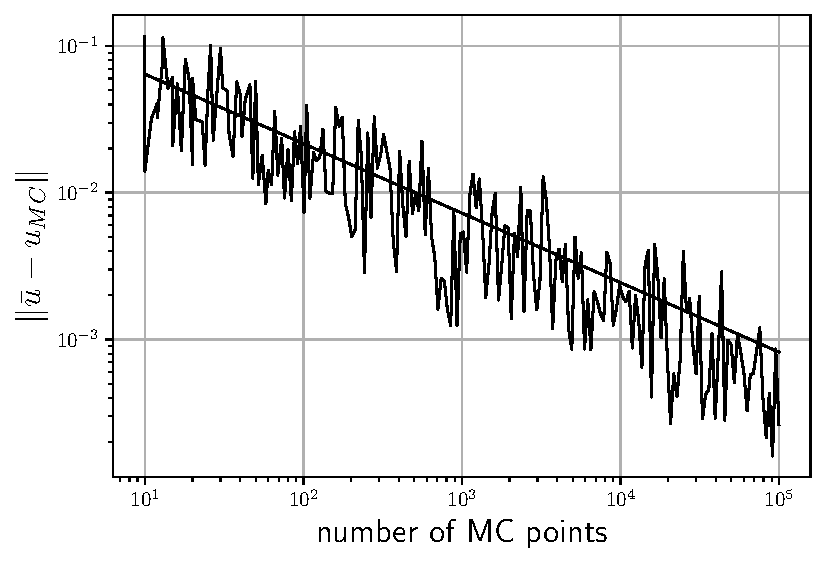
\includegraphics[width=10cm]{pics/MCerrorConv.pdf}
\centering
\caption{Convergence of the error norm for the FEM prior mean}
\end{figure}
\label{fig:u_mean_conv}



\subsection{Step 2: Estimation of Hyperparameters }

Below it was already stated that the hyperparameters for computing the model discrepancy covariance matrix $\bm{C_d}$ are not known. The scaling factor $\rho$ is not known, as well. The measurement data can be used to estimate these parameters, collected in the hyperparameter vector $\bm{w}$, with Bayes' rule 
%
\begin{equation}
p(w|y) = \frac{P(y|w) p(w)}{\int P(y|w) p(w) dw}
\end{equation}
%
where the denominator, which only serves as a normalization constant, can be dropped if only a point estimate of the hyperparameters is needed. This approach is indeed non-bayesian because no probability density of the hyperparameters is computed. For multiple measurements $y_i$ with a total number of $n_o$ there holds, because it is assumed that individual measurements are independent [Rasmussen p.9],
\begin{equation}
P(Y|w) = \prod_{i=1}^{n_o} p(\bm{y_i}) \; 
\end{equation}
which replaces $P(y|w)$.
If no prior knowledge of the parameters is available, it is possible to use an uninformative prior $p(w) = 1$.
The equation then basically states that $p(w|Y) \propto P(Y|w)$ which means that maximizing  $P(Y|w)$, i.e. the likelihood to measure $Y$ given a set of hyperparameters, yields the optimal vector of hyperparameters for the given data. 
The marginal likelihood $P(y|w)$, marginal because ?!?!?!, can be expressed as 
\begin{equation}
p(y|w) = \mathcal{N}(\rho \bm{P}\bar{u}, \bm{C_d}+\bm{C_e} + \rho^2 \bm{P} \bm{C_u} \bm{P}^T)
\end{equation}
because, as stated above, all components of the statistical generating model are Gaussian.
The equation for the corresponding PDF reads
\begin{equation}
p(y|w) = \frac{1}{(2 \pi)^{n/2} |K|^{1/2} } \exp \left(   -\frac{1}{2} (y - \rho \bm{P}\bar{u})^T \bm{K}^{-1} (y - \rho \bm{P}\bar{u})   \right)
\end{equation}
with
\begin{equation}
K = \bm{C_d}+\bm{C_e} + \rho^2 \bm{P} \bm{C_u} \bm{P}^T \; .
\end{equation}
%
To make further calculations easier the exponential function can be removed by taking the negative $\log$ of the function (Rasmussen):
\begin{equation}
- \log p(y|w) = \frac{n}{2} \log(2 \pi) + \frac{1}{2} \log |\bm{K}| + \frac{1}{2}(\rho \bm{P}\bar{u} - y)^T \bm{K}^{-1} (\rho \bm{P}\bar{u} - y) 
\label{eqn:neglog}
\end{equation}
This also improves numerical stability because products of possibly very small factors can become smaller than machine accuracy. The log replaces products with sums.
Because of taking the negative $\log$, (\ref{eqn:neglog}) now needs to be minimized instead of maximized. 

\paragraph{Cholesky Decompositon}
[Gentle 1998 p.93-95]
For numerical stability reasons $\bm{K}^{-1}$ should not be calculated directly. Instead, the linear system is solved. Additionally, if $K$ is symmetric and positive-semidefinite, computing the lower triangular matrix using the Cholesky decomposition 
\begin{equation}
K = LL^T
\end{equation}
makes the calculation quicker and yields the also needed determinant of $K$ as a by-product. 
A generic linear system is defined as $A x = b$. It is solved for $x$, so the inverse of $A$ is needed. In this case for (\ref{eqn:neglog}) there holds $A=K$ and $b = y$, since the inverse of $K$ is meant to be found. Defining $x = K^{-1}y$ there holds
\begin{equation}
K \times K^{-1} \times y = y
\end{equation}
%
With $L$ the lower triangular matrix of $K$ obtained by 
\begin{lstlisting}[language=Python]
L = scipy.linalg.cho_factor(K)
\end{lstlisting}
the linear system can now be solved for $x = K^{-1}y$ with
\begin{lstlisting}[language=Python]
K_inv_y = scipy.linalg.cho_solve(L, y) .
\end{lstlisting}

The determinant of any triangular matrix is defined as the product of its diagonal entries [http://www.math.lsa.umich.edu/~hochster/419/det.html]. Therefore the lower triangular matrix $L$ can be used to efficiently calculate the determinant of $K$. There holds
\begin{equation}
det K = det L det L^T = det L ^2
\end{equation}
and therefore
\begin{equation}
det K = \left(    \prod_{i=1}^{n_y}  L_{i,i}  \right)^2
\label{eqn:CholDet}
\end{equation}

Since in (\ref{eqn:neglog}) the $\log$ likelihood is used, (\ref{eqn:CholDet}) can be simplified to a sum:

\begin{align*}
\log{det K} &= \log{det L}^2 \\
&= 2 \sum_{i=0}^{n_y} \log{L_{i,i}}
\end{align*}

\subsubsection{Minimization of the Negative log-Likelihood}
The best possible set of hyperparameters $\bm{w}$ for (\ref{eqn:neglog}) to be as small as possible has to be found. That can be achieved by using a gradient based optimizer or by sampling the parameter space with, e.g., a MCMC approach.
\paragraph{MCMC}
Markov Chain Monte Carlo (MCMC) is a very efficient sampling method. Just as standard MC, it can be used to draw samples from a given distribution. The advantage of MCMC is now that an algorithm finds a relatively small set of samples which is able to describe the distribution very accurately. The result is a distribution for the hyperparameters of which e.g. the mean can be deduced. One common algorithm is the metropolis algorithm.
The metropolis algorithm is a special case of MCMC for a symmetric proposal distribution.
Metropolis algorithm as code. 



\paragraph{L-BGFS}
L-BGFS is a gradient based optimizer. It doesn't deliver a distribution for the hyperparameters but only a point estimate.
For the optimization with L-BGFS the derivative of (\ref{eqn:neglog}) is needed. It can be computed as follows.





\section{Step 3: Estimating the Optimum Mesh Parameters}


\chapter{Application of statFEM in Vibroacoustics}

\section{Simple 1D example}
\paragraph{Choice of PDE}
The Poisson equation 
%%
\begin{equation}
- \nabla \cdot \mu(x) \nabla u(x) = f(x)
\label{eqn:Poisson}
\end{equation}
%%
is chosen as the governing equation. It is an elliptic partial differential equation (PDE). In this work it is used as a simple 1D example to illustrate how the statistical FEM and especially the Gaussian Process Regression works.
The most standard form of it does not, contrary to this example, include $\mu(x) \in \mathbb{R}^+$ which is the diffusion coefficient dependent on the spatial variable $x$. The right-hand side consists of the source term $f(x)\in \mathbb{R}$. Both $\mu (x)$ and $f(x)$ are the free parameters in this case. The equation is solved for the unknown  $u(x)$ in the domain $\Omega = (0,1)$ with the boundary condition $u(x) = 0$ on $x=0$ and $x=1$.
%
For a first example there holds $\mu(x)=1$. $f(x)$ is modeled as a Gaussian Process [Cirak]
%
\begin{equation}
f(\bm{x}) \sim \mathcal{GP} \left( \bar{f}(\bm{x}), c_f(\bm{x},\bm{x}')\right) \;.
\end{equation}
%
\paragraph{Construction of the GP}
The mean function of the GP is set to $\bar{f}(x) = 1.0$. For the covariance function at first a squared exponential kernel 
%
\begin{equation}
c_f(\bm{x},\bm{x}') =    \sigma_{f}^2 \exp \left(-  \frac{\left \| \bm{x}-{\bm{x}}' \right \|^2}{2l_{f}^2} \right )       
\label{eqn:sqEx_f}
\end{equation}
%
is used with the standard deviation $\sigma_{f} = 0.1$ and the length scale $l_{f} = 0.4$.
In Python the kernel is directly implemented as a function which takes two lists and the parameters as input variables [Murphy]:

%
Here, the parameters are fixed but in a later example a method on how to infer the optimum position for these will be studied.

Having prepared the mean function and the kernel, which can be considered the prior in a GP regression setting, a sample of the GP can be drawn. For this points have to be chosen on which the kernel is evaluated. These are the test points and, according to [Cirak], correspond to the center of the FEM cells. This implies that there are as many test points as FEM cells and therefore the coordinates of the FEM mesh can directly be used to compute the covariance matrix. For that (\ref{eqn:sqEx_f}) is evaluated at $\bm{x} = \bm{x}'$ with $\bm{x}$ the vector of test points. 

A GP has the marginalization property: if you sample it at a finite number of points it yields a multivariate Gaussian distribution $\mathcal{N}(\bar{\bm{f}},\bm{C_f})$ with $\bar{\bm{f}}$ the mean vector and $\bm{C_f}$ the covariance matrix while still describing the underlying continuous sample.
According to [Rasmussen] sampling from a multivariate Gaussian distribution works as follows: To obtain $n$ samples from the prior, at first $n$ samples of a standard normal distribution, also called Gaussian white noise, $e \sim \mathcal{N}(0,1)$ have to be drawn. Computing the Cholesky decomposition of the covariance matrix $\bm{C_f} = LL^T$, which can also be thought of as taking the square root of a matrix, yields the lower triangular matrix $L$. Samples can now easily be drawn from $\bm{f} = \bar{\bm{f}} + Le$ which is a multivariate Gaussian distribution with a mean $\bm{f}$ and a covariance $\bm{C_f}$.

Sample: Normal distribution times std dev. GP with n points is basically a multivariate gaussian with n dimensions. therefore we need the std dev. for a univariate gaussian thats . 

For the observations made in a later step it is assumed that there is some measurement noise. This is modeled as an added variance $\sigma_{n}^2$ on the diagonal of the prior covariance matrix. An additional effect of this added noise is the improved numerical stability of the covariance matrix which is important for computing the Cholesky decomposition.

\section{1D Vibroacoustics Example}
Helmholtz Equation. Looks similar to the Poisson equation but the right side differs. It's the eigenvalue problem for the laplace operator.

\lipsum[2-5] %\cite{campolina}



\chapter{Conclusion and Discussion}

\lipsum[1-3] %\cite{Langer2019}

\section{Section 1}

\lipsum[4-7] %\cite{Yaghoubi:2017}


\begin{thebibliography}{4}
%
\bibitem{campolina}
Campolina, B.: Vibroacoustic modelling of aircraft double-walls with structural links using Statistical
Energy Analysis (SEA). Acoustics [physics.class-ph]. Université de Sherbrooke; Université Pierre
et Marie Curie - Paris VI (2012)

\bibitem{Langer2019}
Langer, S.C., Blech, C.: Cabin noise prediction using wave‐resolving aircraft models. Proc. Appl. Math. Mech., Vol. 12 (1) (2019): e201900388. doi:10.1002/pamm.201900388

\bibitem {Yaghoubi:2017} Yaghoubi, V., Marelli, S., Sudret, B., Abrahamsson, T.: Sparse polynomial chaos expansions of frequency response functions using stochastic frequency transformation, Probabilistic Engineering Mechanics, volume 48, pages 39-58 (2017)
\end{thebibliography}

\end{document}
